\clearpage
\section{Régression logistique régularisé}

\subsection{Visualisation des données}
\begin{figure}[!h]
    \begin{minipage}{.48\linewidth}
        Après avoir éxecuter la fonction d'affichage des données on constate ici que nous n'aurons pas une limite de décision linéaire dû à l'allure circulaire. \\
        On ne peut donc pas se limité à $x_1$ et $x_2$. Nous allons mapper les caratéristiques sour forme de termes polynomiaux jusqu'à la puissance 6 pour obtenir un 
        vecteur de dimension 28 grâce à nos deux caractéristiques. \\
        La multiplication des caractéristiques nous permettra d'obtenir une régularisation logistique cohérente avec nos échantillons.

    \end{minipage}\hfill
    \begin{minipage}{.48\linewidth}
        \begin{center}
            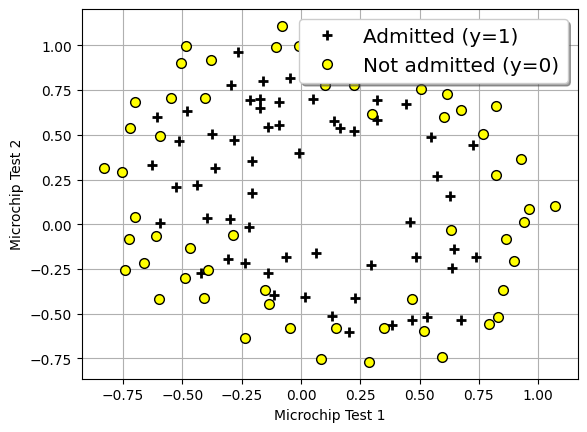
\includegraphics[width=1\textwidth]{./img/4.1.png}
            \caption{\label{fig:4.1}Visualisation des données}  
        \end{center}
    \end{minipage}
\end{figure}

Cependant, plus il y a de caractéristiques, plus la limite décision est fidèle à nos échantillons. Ce problème est appelé l'\textit{overfitting}, les conséquences sont des prédictions futures 
incorrectes. \\
Pour contrer le sur-apprentissage nous allons mettre en place une régularisation et modifier ses paramètres pour constater l'intérêt de régulariser notre fonction de coût $J(\theta)$ et 
la descente de gradient suite à un nouveau mappage.

\subsection{Fonction de coût régularisé $J(\theta)$}

\begin{equation}\label{eq:cout-reg}
    J(\theta) = \frac{1}{m} \sum_{i=0}^{m-1}[-y^{(i)} log(h_\theta(x^{(i)})) - (1-y^{(i)}) log(1-h_\theta(x^{(i)}))] \underbrace{+ \frac{\lambda}{2m} \sum_{j=1}^{n-1} \theta_j^2}_{(a)}
\end{equation}

\begin{itemize}
    \item [(a)] La régularisation nous permet d'atténuer tout les coefficient $\theta$ en fonction du paramètre $\lambda$. Plus celui-ci est petit, plus $\theta$ sera atténué.
\end{itemize}

\begin{figure}[!h]
\begin{minted}[frame=lines, framesep=2mm, baselinestretch=1.2, fontsize=\footnotesize, linenos, breaklines=true]{python}
def costFunctionReg(theta, X, y, Lambda):
    theta = theta.reshape((n,1)) # due to the use of fmin_tnc
    predictions = sigmoid(X @ theta)
    J = (1/m) * np.sum(-y * np.log(predictions) - (1 - y) * np.log(1 - predictions)) + ((Lambda/(2*m)) * np.sum(theta[1:]**2))
          
    return J

    """return 
    Cost at initial theta (zeros): 0.693147
    Expected cost (approx): 0.693
    -------------------------- 
    Cost at test theta (with lambda = 10): 3.164509
    Expected cost (approx): 3.16
    """
\end{minted}   
\captionof{listing}{Fonction de coût régularisé}
\end{figure}
    


\subsection{Descente de gradient régularisé}

\begin{align}\label{eq:descente-gradient-reg}
    \frac{\partial J(\theta)}{\partial \theta_j} = \frac{1}{m} \sum_{i=0}^{m} (h_\theta(x^{(i)}) - y^{(i)}) x_j^{(i)} \qquad \qquad \qquad \text{pour} \quad j=0 \\
    \frac{\partial J(\theta)}{\partial \theta_j} = \frac{1}{m} \left( \sum_{i=0}^{m} (h_\theta(x^{(i)}) - y^{(i)}) x_j^{(i)} + \underbrace{\lambda \theta_j}_{(a)} \right) \qquad \qquad \qquad \text{pour} \quad j\geq1 
\end{align}

\begin{itemize}
    \item [(a)] Ici, on adapte également la régularisation sur la descente de gradient comme pour le coût $J(\theta)$. Conventionnellement on ne régularise pas $\theta_0$
\end{itemize}

\begin{figure}[!h]
\begin{minted}[frame=lines, framesep=2mm, baselinestretch=1.2, fontsize=\footnotesize, linenos, breaklines=true]{python}
def gradientFunctionReg(theta, X, y, Lambda):
    m,n = X.shape   # number of training examples and parameters
    theta = theta.reshape((n,1)) # due to the use of fmin_tnc
    grad = 0
    for i in range(m):
            grad += (1/m) * (sigmoid(X[i] @ theta) - y[i]) * X[i]

    grad[1:] += (Lambda/m * theta.flatten()[1:])

    return grad

    """return 
    Gradient at initial theta (zeros):[8.4745e-03 1.8788e-02 7.77711-05 5.0344e-02 1.1501e-02]
    Expected gradients (approx): 8.5e-03 1.88e-02 7.7e-05 5.03e-02 1.15e-02
    -------------------------- 
    Gradient at test theta: [0.3460 0.1613 0.1947 0.2268 0.0921]
    Expected gradients (approx): 0.3460 0.1614 0.1948 0.2269 0.0922
    """
\end{minted}   
\captionof{listing}{Fonction de coût régularisé}
\end{figure}


\subsection{Tracé de la limite de décision}

\begin{figure}[!h]
    \begin{minipage}{.48\linewidth}
       On trace la limite de décision avec \textit{plotDecisionBoundary} après avoir minimiser les valeurs de $\theta$ à l'aide la descente de gradient régularisée. \\
       Le facteur de régularisation $\lambda$ est de 1, ce qui semble convenable. Notre limite de décision inclue la majorité des admis et exclus la majorité des refus. \\

       Nous pouvons donc considérer que le modèle appris par ce classificateur est correct.

    \end{minipage}\hfill
    \begin{minipage}{.48\linewidth}
        \begin{center}
            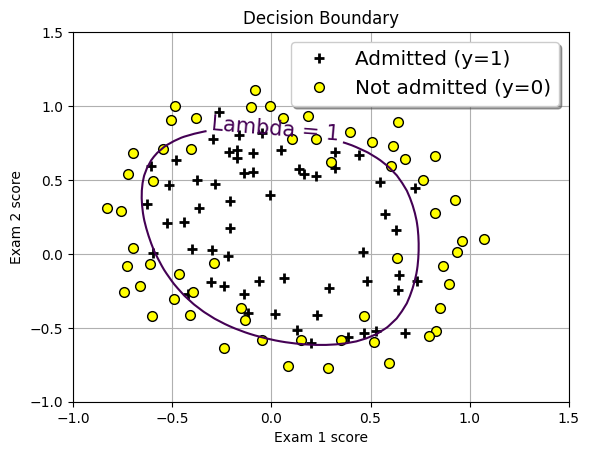
\includegraphics[width=1\textwidth]{./img/4.4.png}
            \caption{\label{fig:4.4}Tracé de la limite de décision}  
        \end{center}
    \end{minipage}
\end{figure}


\subsection{Impacte de $\lambda$}

\begin{figure}[!h]
    \begin{minipage}{.48\linewidth}
        \begin{center}
            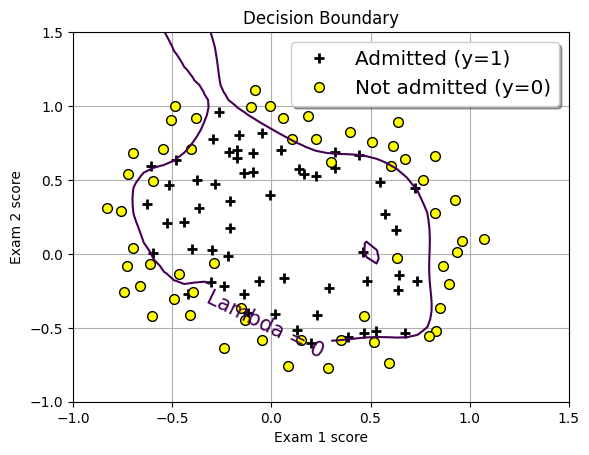
\includegraphics[width=1\textwidth]{./img/4.5(1).png}
            \caption{\label{fig:4.5(1)}Limite de décision avec $\lambda=0$}  
        \end{center}
    \end{minipage}\hfill
    \begin{minipage}{.48\linewidth}
        \begin{center}
            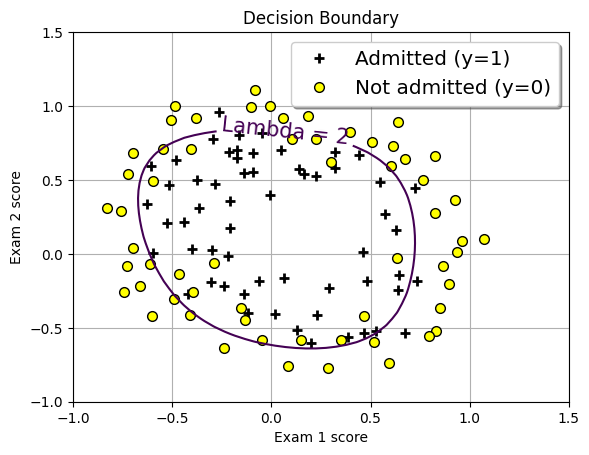
\includegraphics[width=1\textwidth]{./img/4.5(2).png}
            \caption{\label{fig:4.5(2)}Limite de décision $\lambda=2$}  
        \end{center}
    \end{minipage}
\end{figure}

\begin{figure}[!h]
    \begin{minipage}{.48\linewidth}
        \begin{center}
            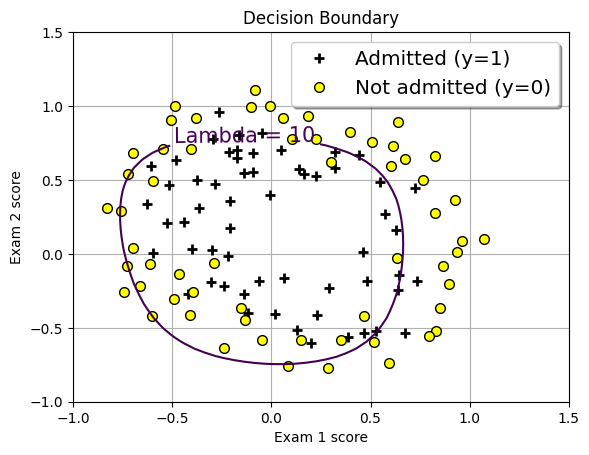
\includegraphics[width=1\textwidth]{./img/4.5(3).png}
            \caption{\label{fig:4.5(3)}Limite de décision avec $\lambda=10$}  
        \end{center}
    \end{minipage}\hfill
    \begin{minipage}{.48\linewidth}
        \begin{center}
            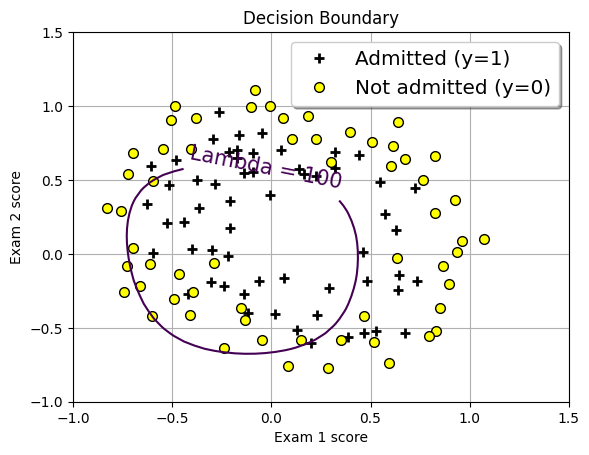
\includegraphics[width=1\textwidth]{./img/4.5(4).png}
            \caption{\label{fig:4.5(4)}Limite de décision $\lambda=100$}  
        \end{center}
    \end{minipage}
\end{figure}

Les 4 courbes nous permettent de visualiser l'impacte de $\lambda$. \\
Comme expliqué plus tôt, un nombre important de caractéristiques sans régularisation nous permettent d'obtenir un modèle proche des échantillons. La figure \ref{fig:4.5(1)}, montre que c'est bien le 
cas puisque le facteur de régularisation est nul. On imagine facilement que les prédictions ne peuvent pas être concluantes puisqu'on assiste au problème de sur-apprentissage. \\
D'un autre côté quand le facteur de régularisation est trop important, le modèle n'est pas suffisament précis. Ce qui implique un sous-apprentissage.
